\section{Computer Simulations} \label{simulations}

\subsection{LTspice Simulations}
Since the 4-quadrant operation and control of the H-Bridge topology is not simple, we made comprehensive simulations using LTspice.A brief description of those and their results will be explained in this subsection. First, the simulation model will be described. \\

The model for the topology we are using is given in Figure \ref{fig:LTspice_topology_sch}. MOSFET models are chosen from the libraries of LTspice, whose ratings are compatible with our operation ranges. To simulate the rectified DC voltage on the input side, we occasionally used an ideal DC source to simplify the results by avoiding the input voltage ripple. We used a diode to model the one-directional current flow of the rectifier, and a capacitor to model the output filtering capacitor of the rectifier. The chopper and the H-Bridge is model is rather straightforward.

\begin{figure}[H]
    \centering
    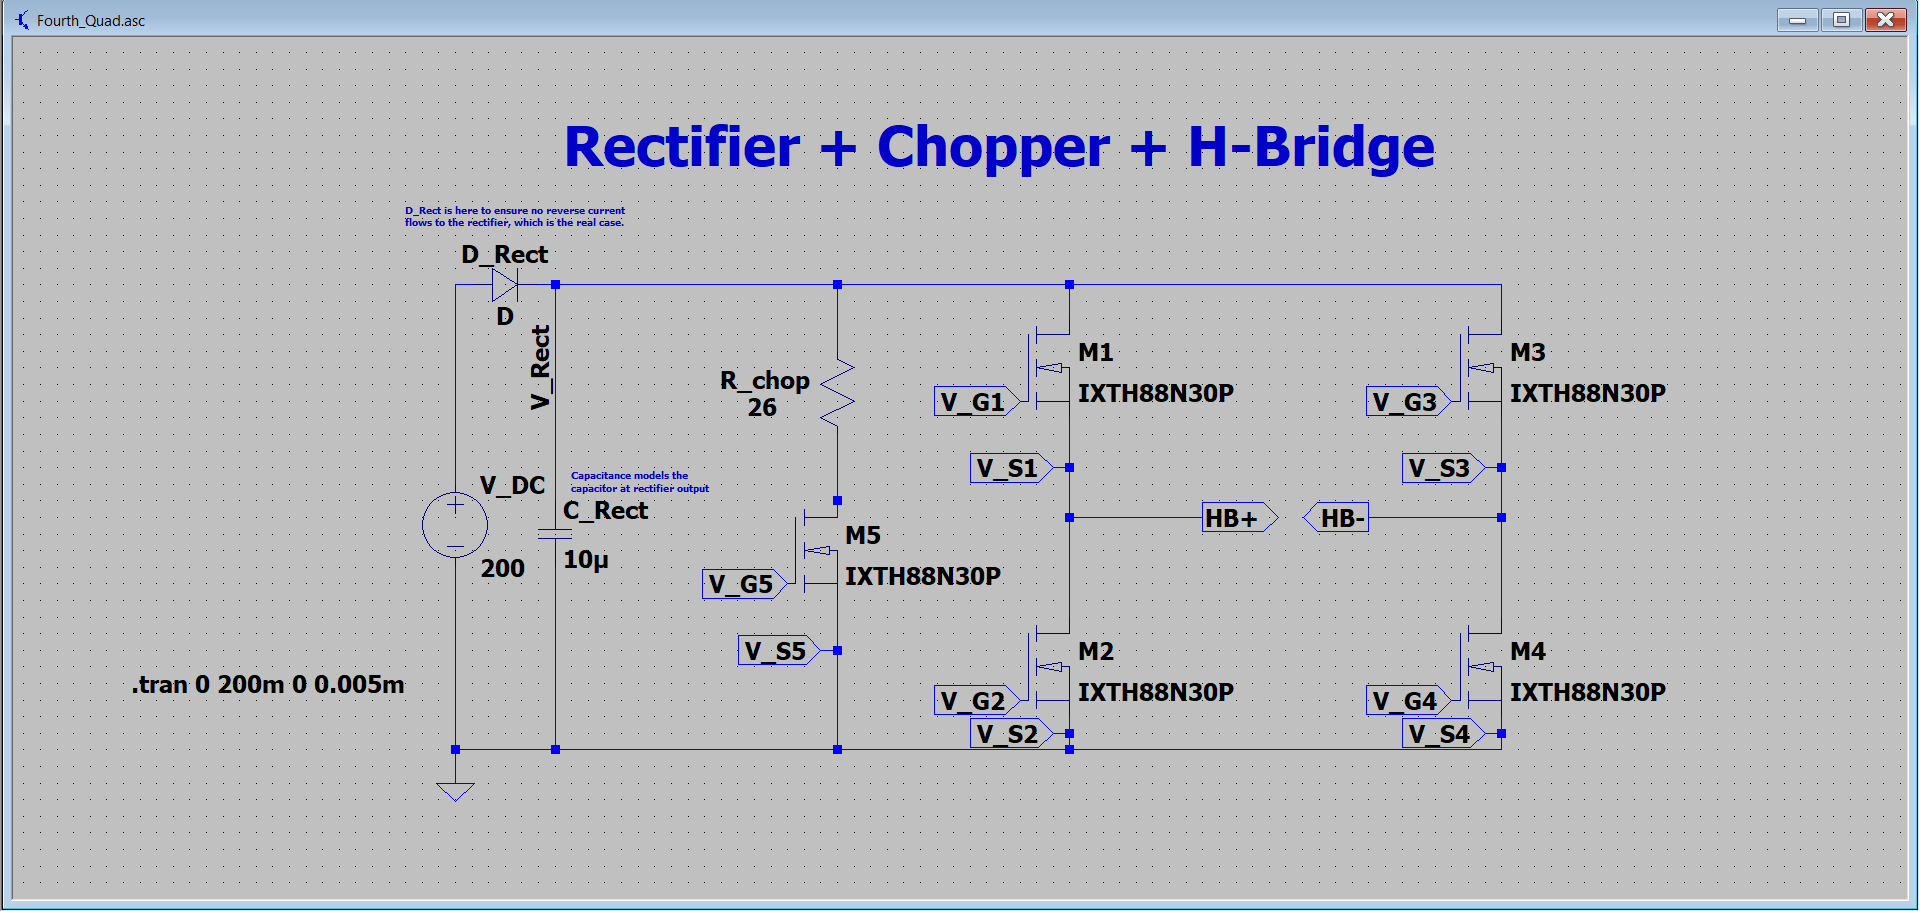
\includegraphics[width=0.8\textwidth]{Figures/Spice_Figures/Schematics/Rectifier_Chopper_H-Bridge_Schematic.PNG}
    \caption{Simulation model for the 4-quadrant motor driver topology we choose}
    \label{fig:LTspice_topology_sch}
\end{figure}

The controller and gate driver sections in Figure \ref{fig:LTspice_driver_controller_sch} are modeled using behavioral and usual voltage sources to create the necessary gate to source voltages.

\begin{figure}[H]
    \centering
    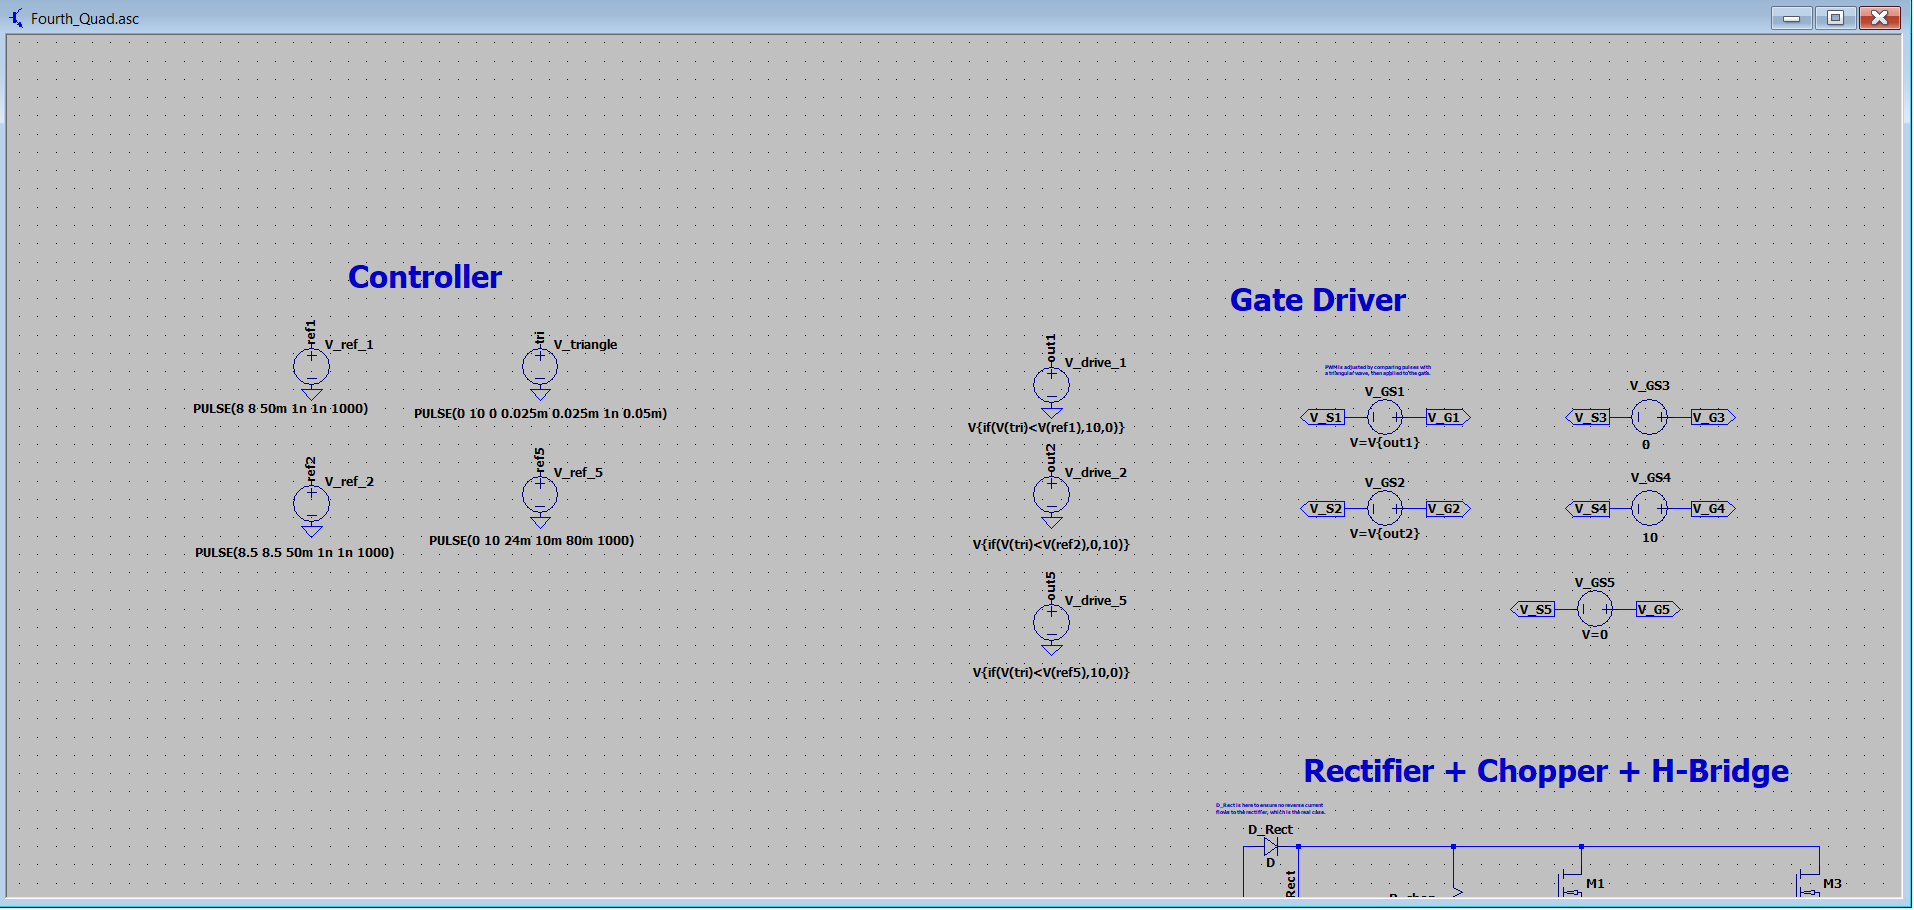
\includegraphics[width=0.8\textwidth]{Figures/Spice_Figures/Schematics/Gate_Driver_Controller_Schematic.PNG}
    \caption{A simple model to simulate the gate driver and controller operation}
    \label{fig:LTspice_driver_controller_sch}
\end{figure}

The electromechanical simulation models for DC motors are given in Figure \ref{fig:LTspice_motor_sch}. Since the simple model of the DC motor is also LTI (Linear Time Invariant), we can simulate it using the LTI circuit which is built and shown in the figure. The model can be derived using the mechanical laws for rotational systems, the torque and back emf formulas of the DC motor models, and Kirchoff's circuital laws. The motor parameters are not the final values, but found iteratively to simulate the DC motor we used as realistically as possible. Note that another DC machine is coupled to our DC machine which is going to be the The overall model for the LTspice simulations is given in Figure \ref{fig:LTspice_whole_sch}.

\begin{figure}[H]
    \centering
    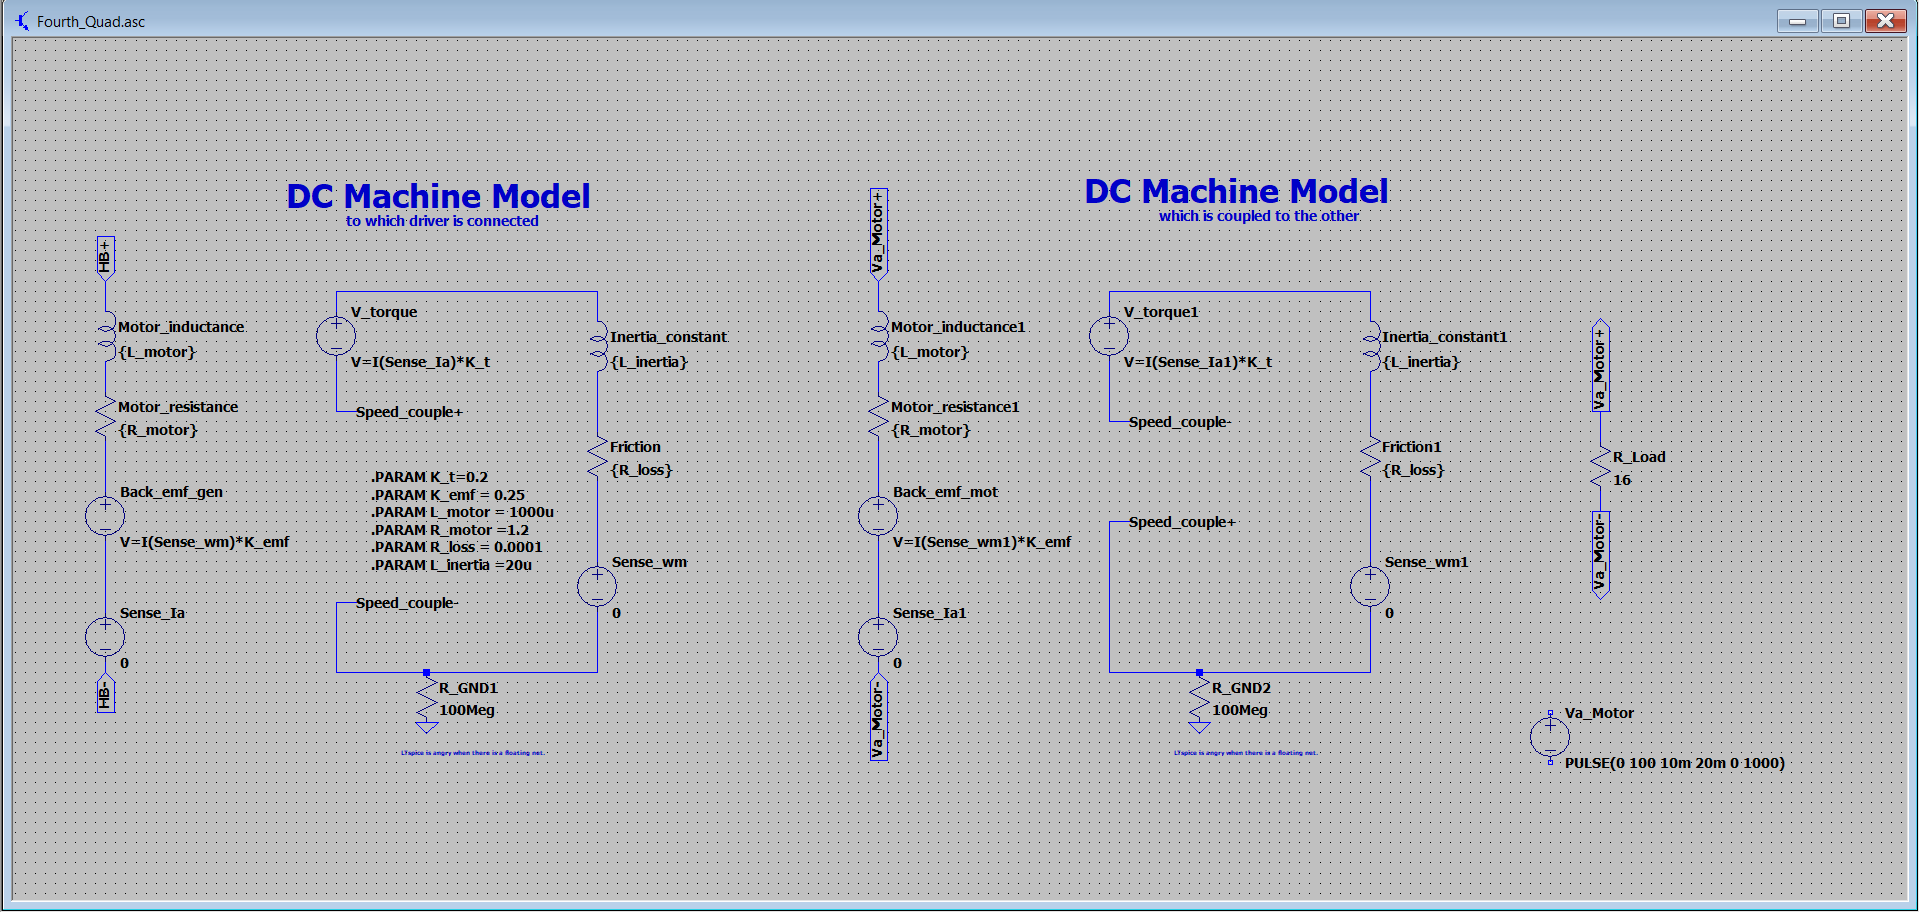
\includegraphics[width=0.8\textwidth]{Figures/Spice_Figures/Schematics/DC_Motor_Models_Schematic.PNG}
    \caption{Electromechanical simulation model for DC motors}
    \label{fig:LTspice_motor_sch}
\end{figure}

\begin{figure}[H]
    \centering
    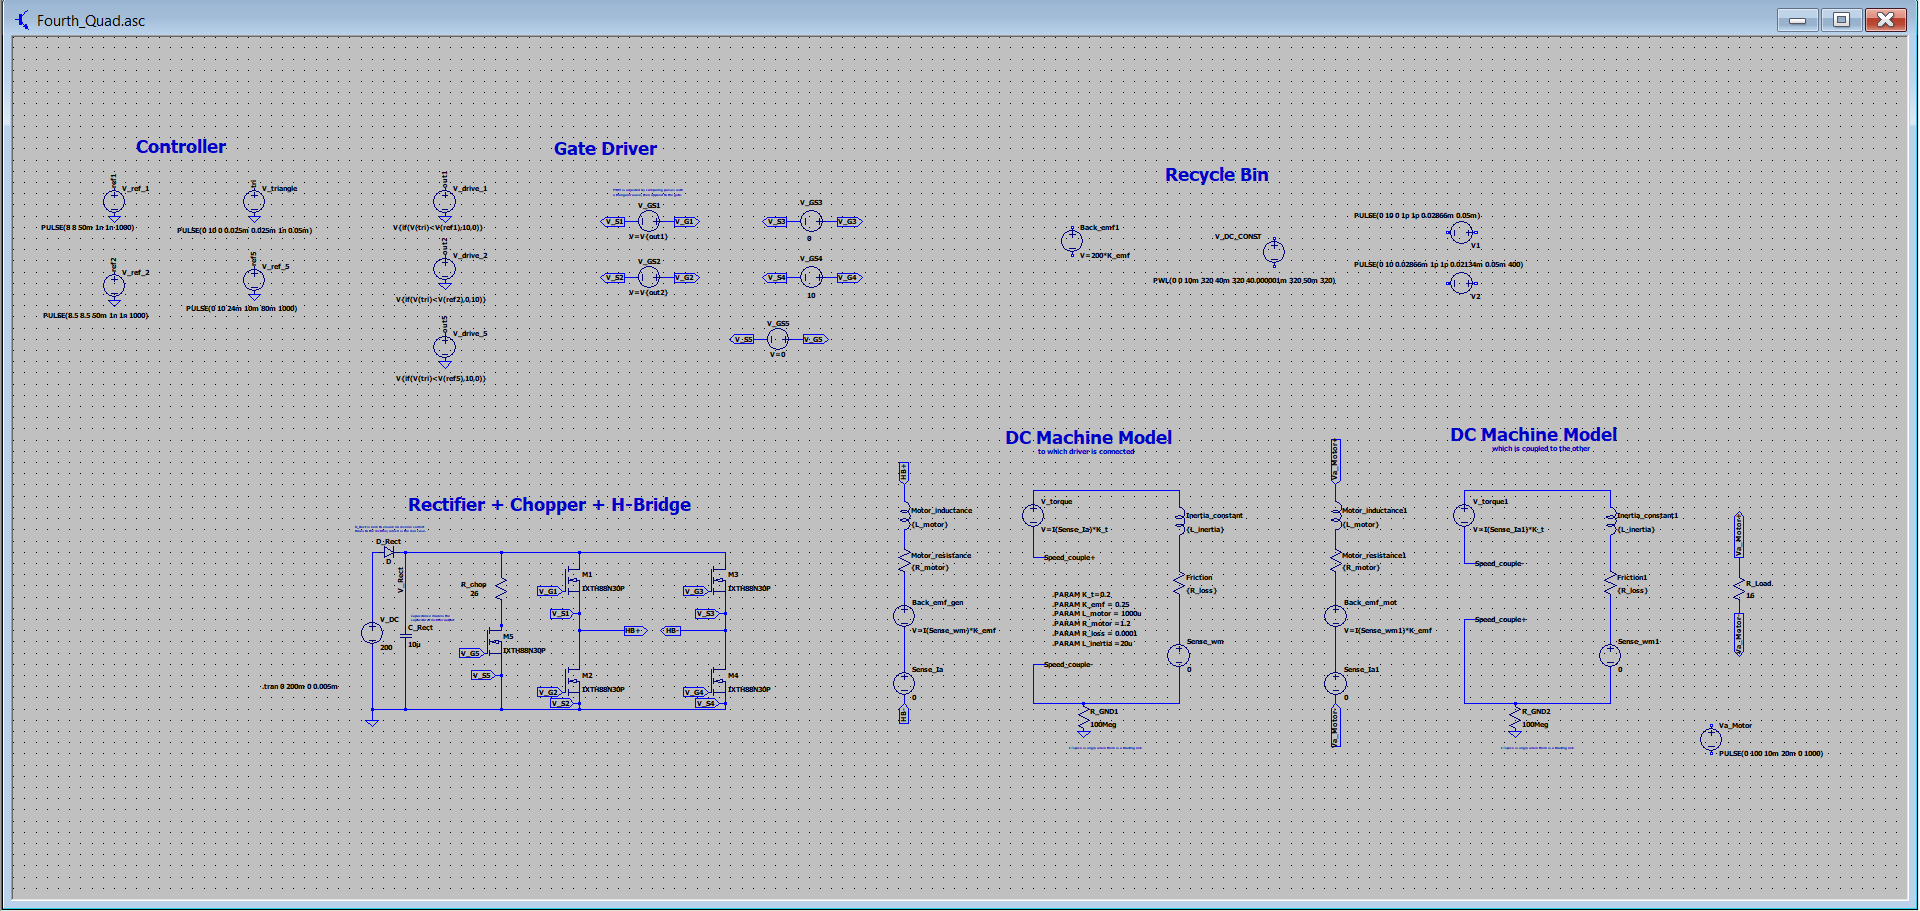
\includegraphics[width=0.8\textwidth]{Figures/Spice_Figures/Schematics/Whole_Model_Schematic.PNG}
    \caption{The complete simulation model used for the DC motor drive simulations in LTspice}
    \label{fig:LTspice_whole_sch}
\end{figure}

For the forward motoring region simulations, M1 and M2 MOSFETs are used for switching, M3 is always off, and M4 is always on for H-Bridge to operate as a synchronous buck converter. The output voltage level is directly proportional with the duty cycle of M1. For example, for 90\% duty, we obtain 180V average voltage on the motor terminals, and we obtain 100V for 50\% duty. These cases are simulated and shown in Figures \ref{fig:LTspice_forward_90_duty} and \ref{fig:LTspice_forward_50_duty}. The current on the 16 $\Omega$ load, the armature current, and the voltage on the H-Bridge terminals are given in the figures. Note that for these values, one can supply more than 2kW power with the motor driver. Hence, current and voltage ratings of the MOSFETs can be determined using such a simulation (keeping the other practical effects in mind).

\begin{figure}[H]
    \centering
    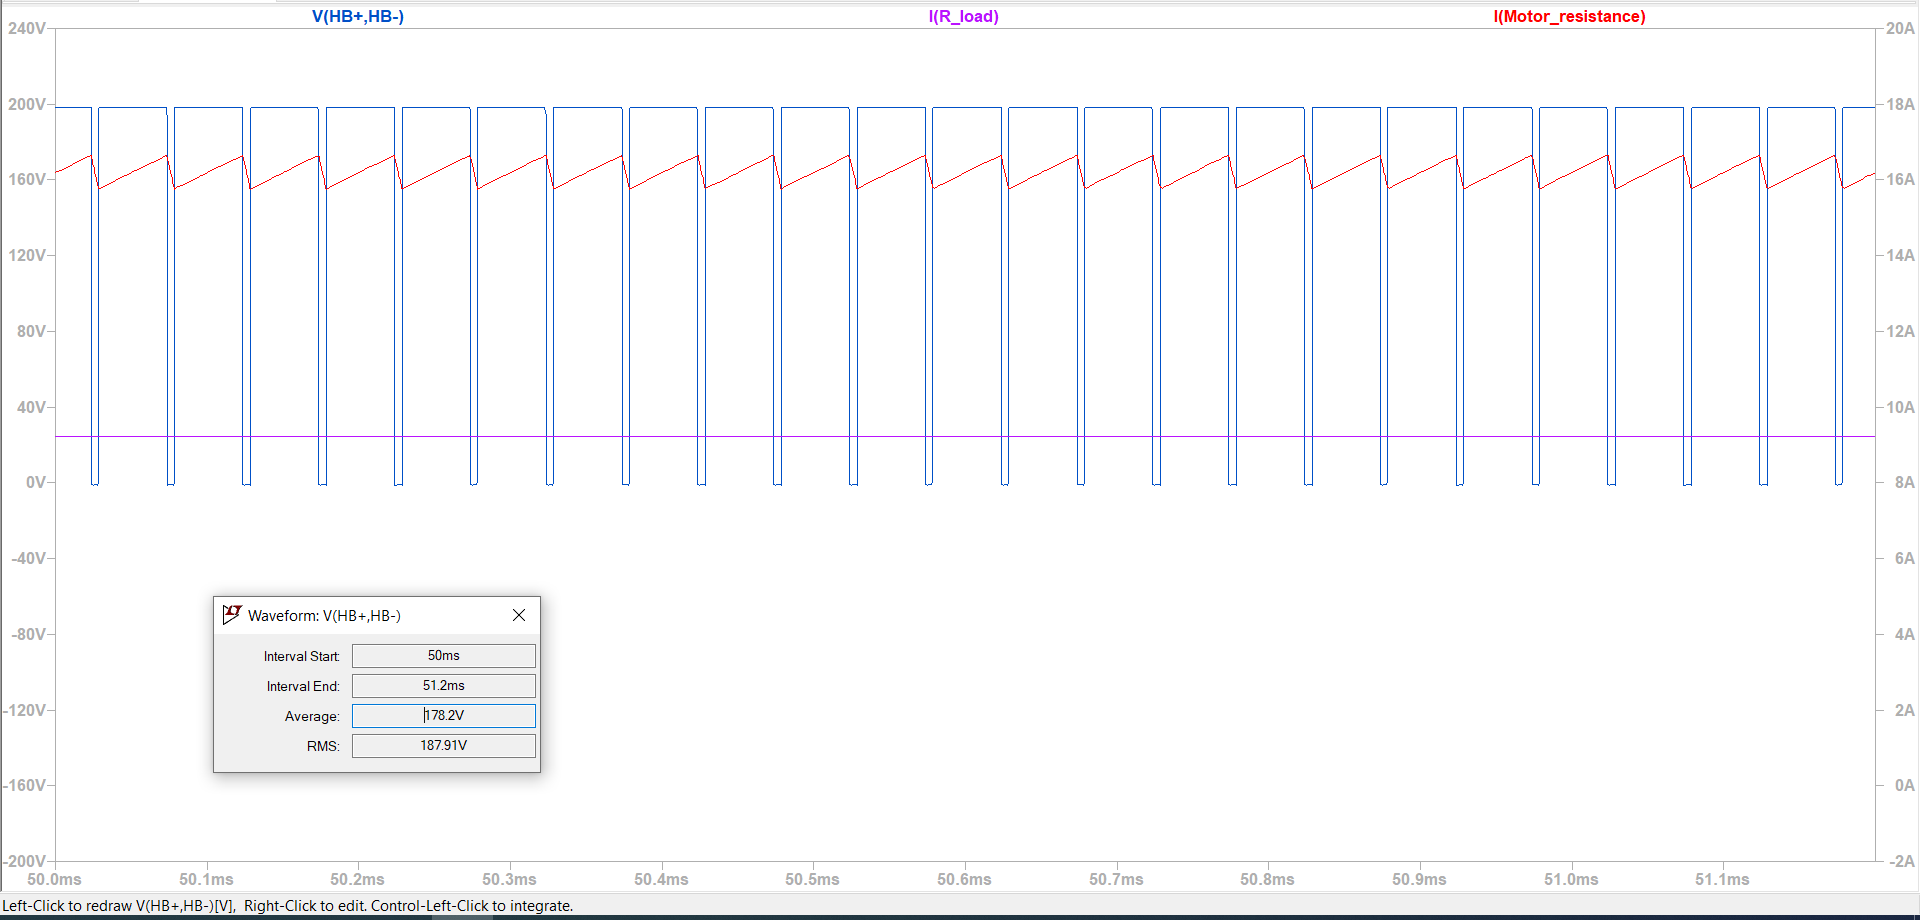
\includegraphics[width=0.8\textwidth]{Figures/Spice_Figures/Motoring_Full_Duty_Sim_1.PNG}
    \caption{Forward motoring simulation for 90\% duty}
    \label{fig:LTspice_forward_90_duty}
\end{figure}

\begin{figure}[H]
    \centering
    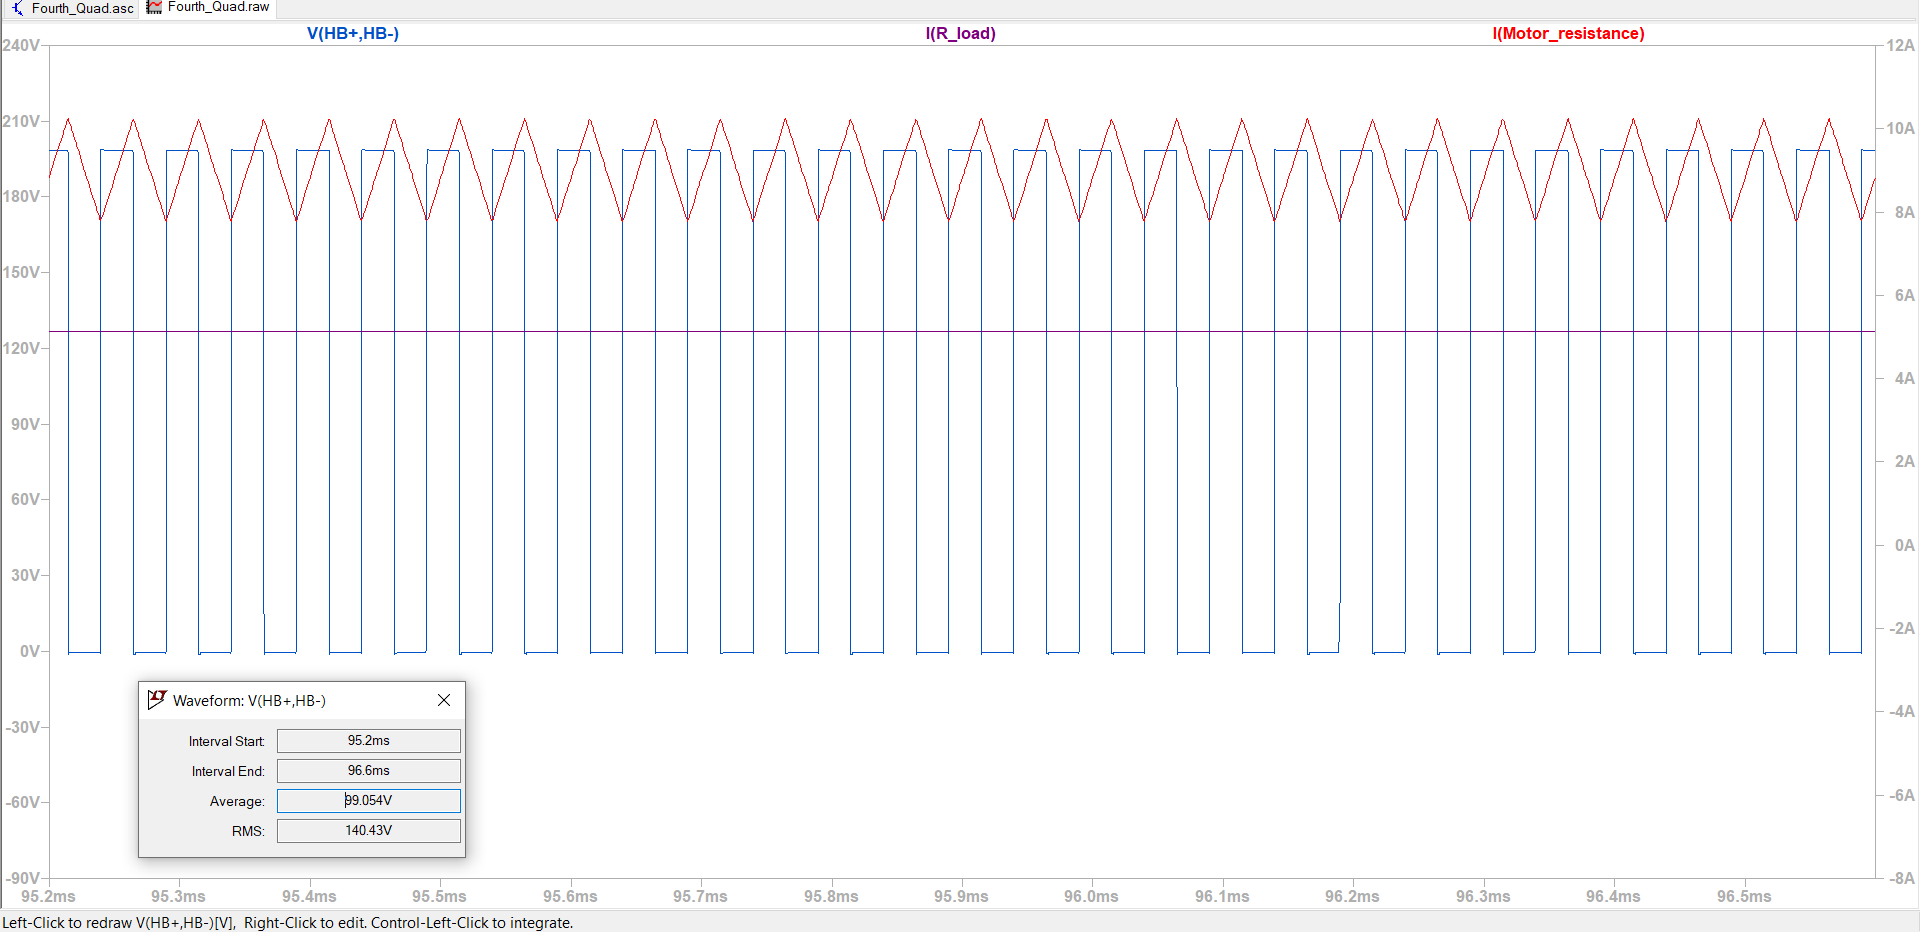
\includegraphics[width=0.8\textwidth]{Figures/Spice_Figures/Motoring_Half_Duty_Sim_1.PNG}
    \caption{Forward motoring simulation for 50\% duty}
    \label{fig:LTspice_forward_50_duty}
\end{figure}

All these simulations are also done with a rectified input, which is coming from a three phase full bridge rectifier. Forward motoring simulation results for the rectified input voltage is given in Figure \ref{fig:LTspice_forward_90_duty_rectified}. Note that there is a significant current ripple in steady state, which is not desired. This will be avoided by the closed loop PID current control by changing the duty according to the input voltage.\\

The average power plots for the output of the driver and one of the switching MOSFETs (M1) are given in Figure \ref{fig:LTspice_forward_90_duty_rectified_power}. The average power consumed by the MOSFET is also calculated and found to be around 10W. This value does not accurately model the real losses, but still gives an idea about the order of magnitude of the MOSFET losses, which is very satisfying for this simulation. In future simulations, more realistic thermal models and simulations will be made.

\begin{figure}[H]
    \centering
    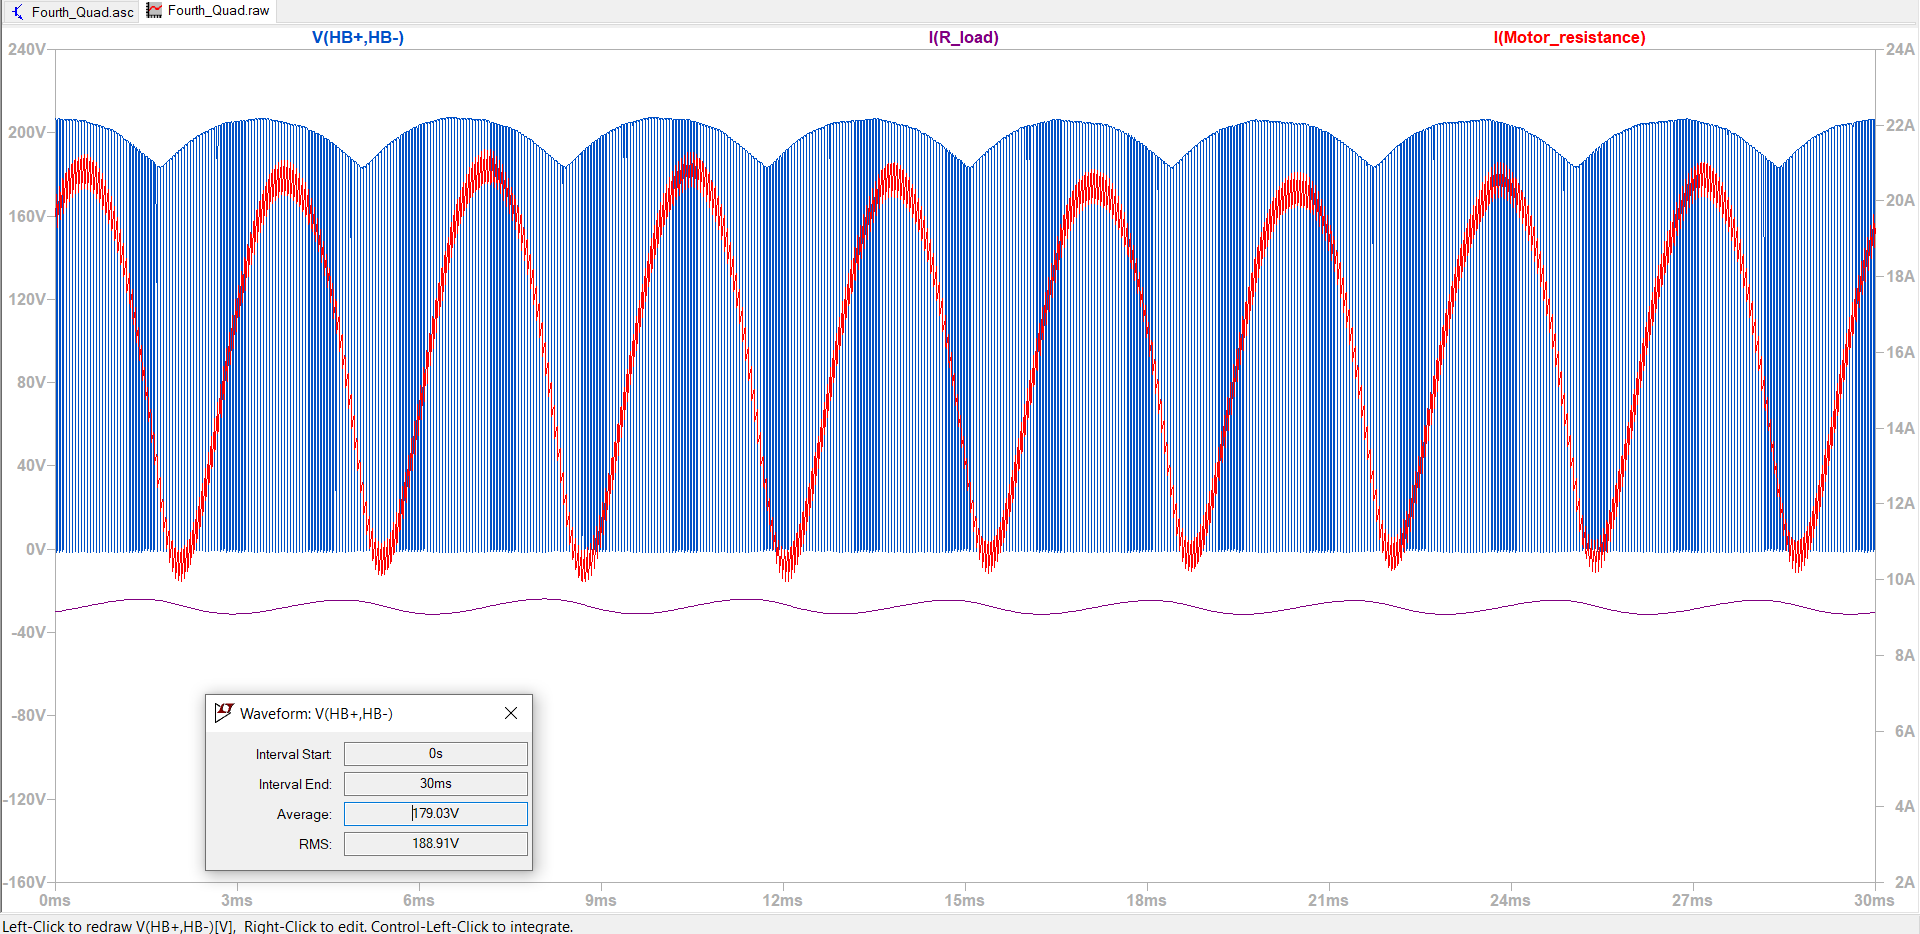
\includegraphics[width=0.8\textwidth]{Figures/Spice_Figures/Motoring_Full_Duty_Rectified_Sim.PNG}
    \caption{Forward motoring simulation for 90\% duty with rectified input}    \label{fig:LTspice_forward_90_duty_rectified}
\end{figure}

\begin{figure}[H]
    \centering
    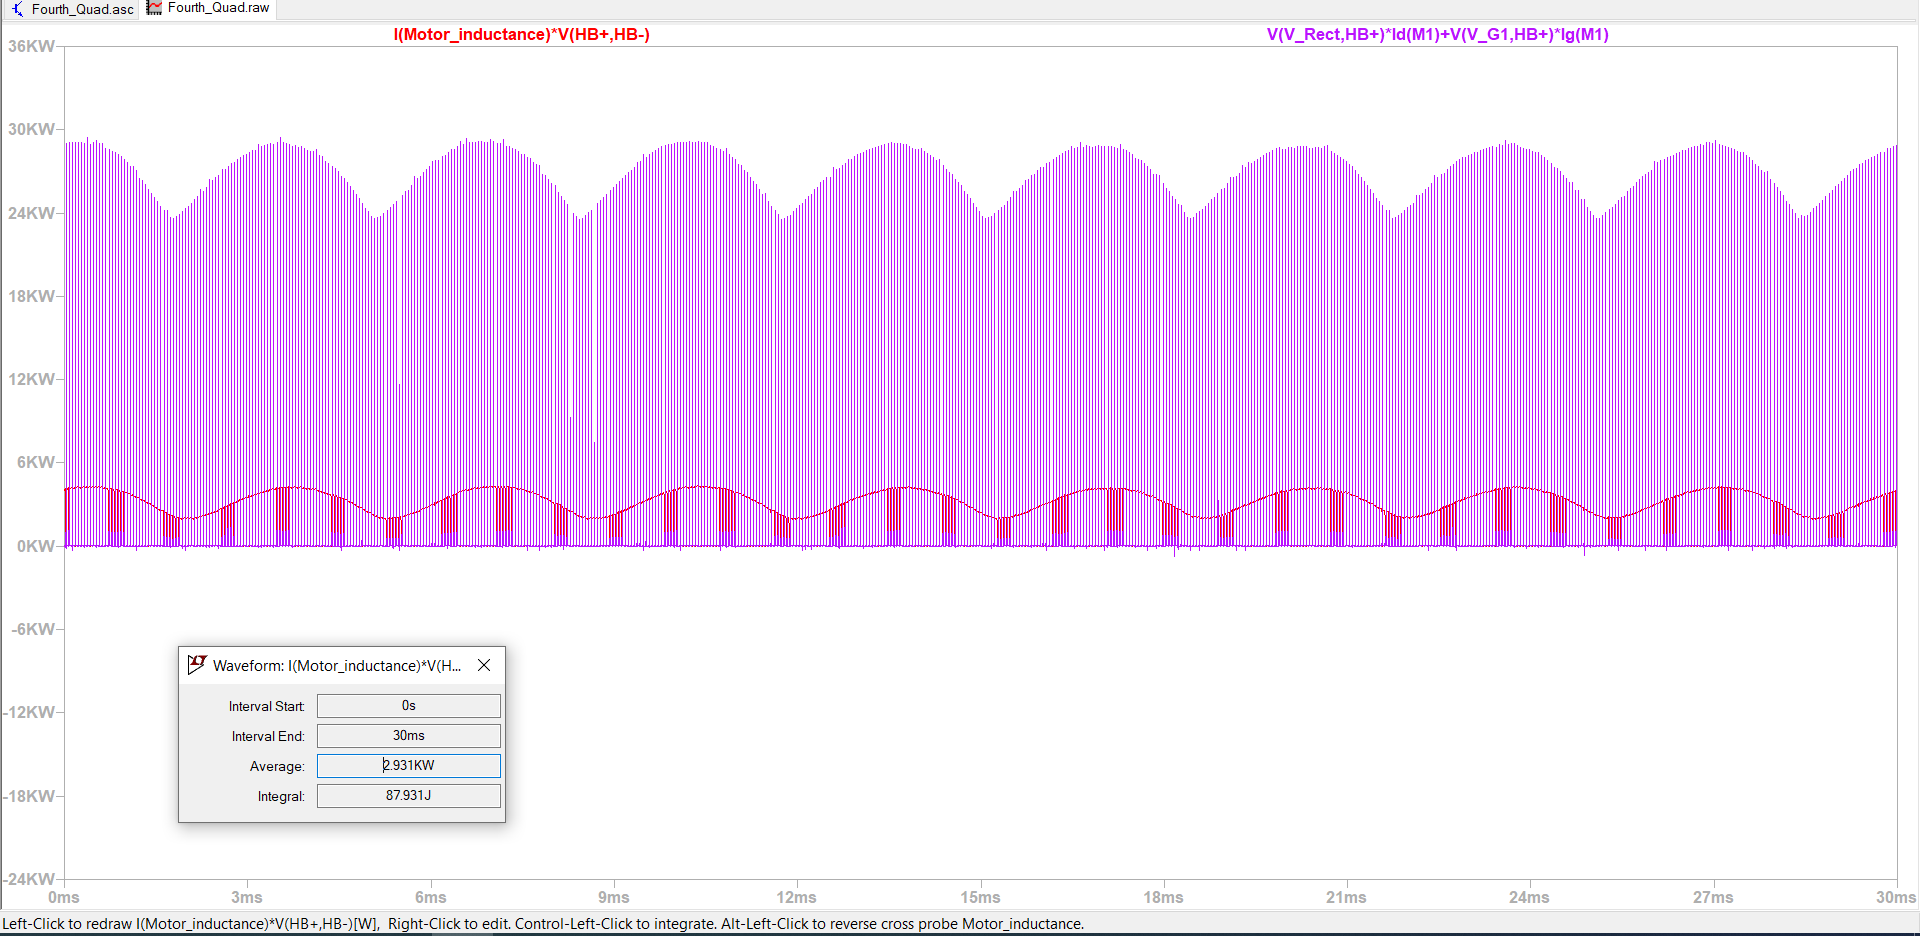
\includegraphics[width=0.8\textwidth]{Figures/Spice_Figures/Motoring_Full_Duty_Rectified_Losses_MOSFET10W_Sim.PNG}
    \caption{Forward motoring simulation for 90\% duty with rectified input, power plots}
    \label{fig:LTspice_forward_90_duty_rectified_power}
\end{figure}

For testing both the forward motoring and regenerative breaking, we made a simulation in which we suddenly change the duty from 90\% to 50\%. This will try to slow down the motor and the motor will release its dissipate its kinetic energy by supplying power to the driver. At this moment, since we did not switch on the chopper resistor in the simulation, the capacitor on the input side is charged to a large value. The transient response is seen in Figure \ref{fig:LTspice_regenerative_breaking}. Note that when our current sensor senses the reverse current, the micro-controller will switch the chopper resistor on and the energy will be dissipated on the resistor.

\begin{figure}[H]
    \centering
    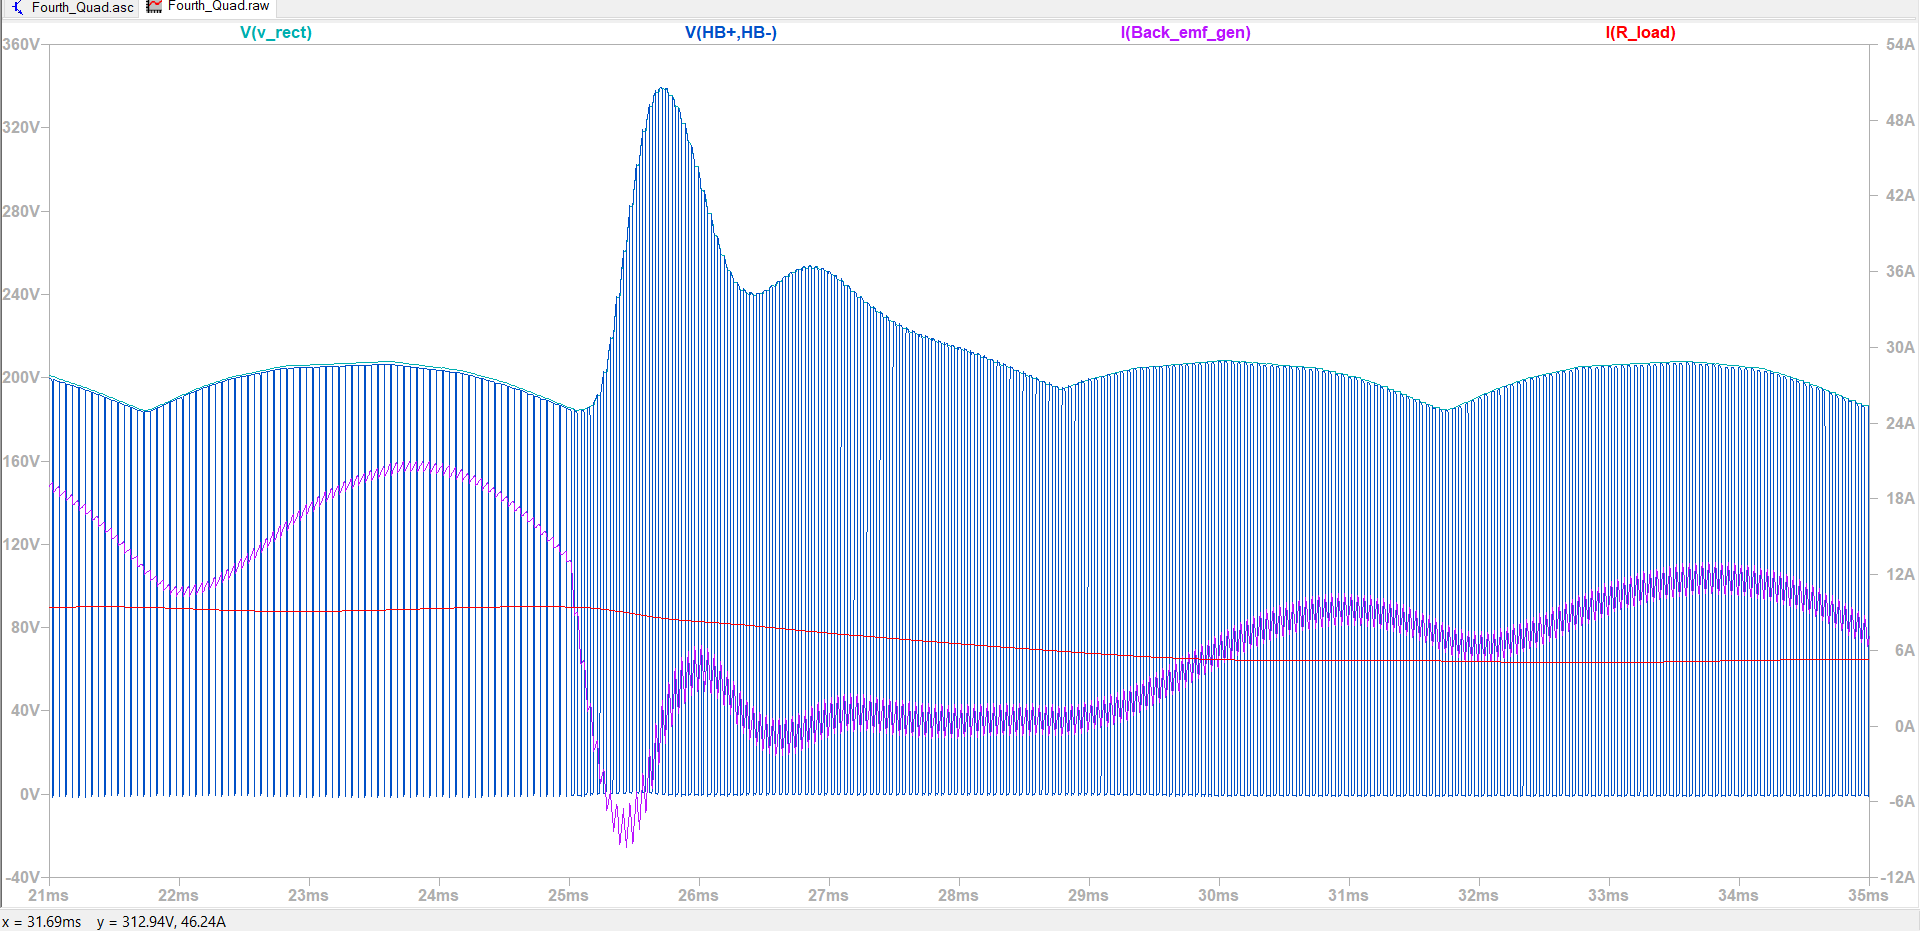
\includegraphics[width=0.8\textwidth]{Figures/Spice_Figures/Motoring_Full_Duty_to_Half_Regenerative_Sim.PNG}
    \caption{Regenerative breaking simulation for sudden slow down (transient)}    
    \label{fig:LTspice_regenerative_breaking}
\end{figure}

The same simulations are run for the reverse motoring operation (M1 off, M2 on, M3 and M4 switched for a synchronous buck with inverted output voltage). The results were similar to the forward motoring case, except for the directions of the currents and voltages on the armature side, which was expected. \\

Finally, the continuous operation in the generation mode is tested by supplying a higher voltage to the other motor. In this operation, none of the MOSFETs are switched on except the chopper switch. The current flow is permitted by the body diodes of the MOSFETs. In the real case, M1 and M4 can be switched to increase the efficiency, but no need to simulate that case. Chopper MOSFET is switched on after 1ms the other motor starts to rotate. The simulation results are given in Figure \ref{fig:LTspice_generation}. One can see that the armature current is negative after the transient, hence supplied to the driver; and the chopper current is positive. These are the desired transient and steady responses of the generation mode and the results are as expected. \\

\begin{figure}[H]
    \centering
    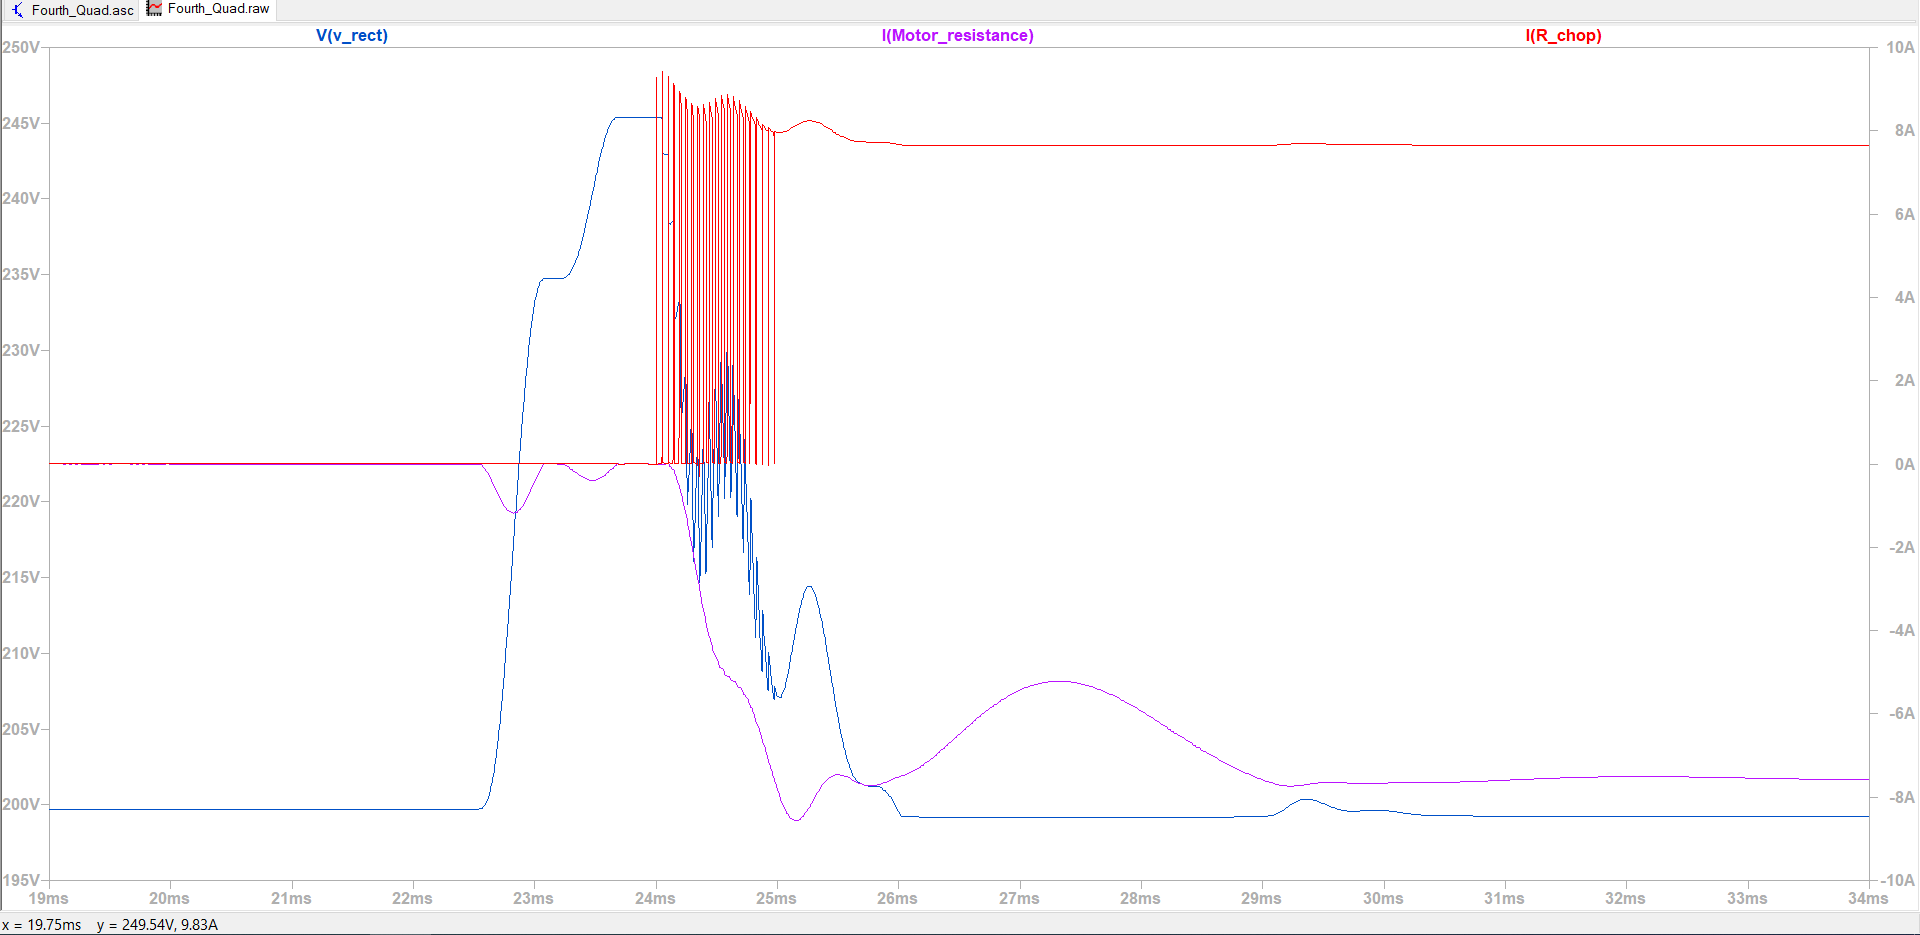
\includegraphics[width=0.8\textwidth]{Figures/Spice_Figures/Generating_Mode_Start.PNG}
    \caption{Continuous generation mode simulation}   
    \label{fig:LTspice_generation}
\end{figure}

In the next steps, we need to consider the inductances and resistances caused by the copper tracks of the PCB layout, which will cause unwanted effects. The realistic models of the components we choose will also be included in the simulations to get better results. Finally, thermal simulations will be conducted according to the directives given by the component manufacturers to further investigate the thermal properties of the system. We continuously update and iterate our simulations to obtain a better view of the electrical, thermal, and mechanical systems considered in our project. For now, we have seen that using H-Bridge topology, we can operate our DC motor in all 4-quadrants with great success.


\subsection{MATLAB Simulations}
Expected circuitry is simulated using MATLAB/Simulink environment. The first stage is added as a three-phase full-bridge rectifier. After that H-bridge and motor simulations are added to have a complete simulation. Simulation setup can be seen in Figures \ref{fig:matlab_model1} \&
\ref{fig:matlab_model2}.

\begin{figure}[ht]
    \centering
    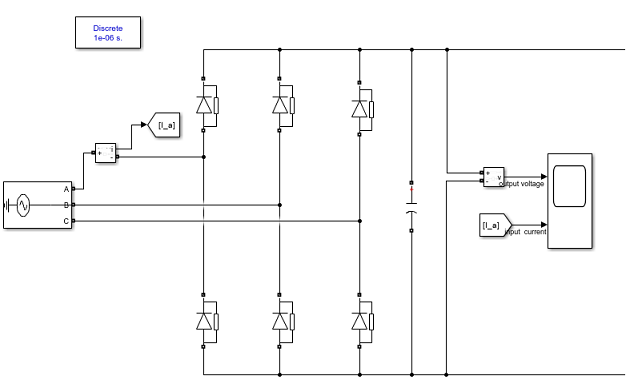
\includegraphics[width=0.8\textwidth]{matlab/MATLAB_model_rect.png}
    \caption{MATLAB Simulation Model Three-Phase FBDR.}
    \label{fig:matlab_model1}
\end{figure}

\begin{figure}[ht]
    \centering
    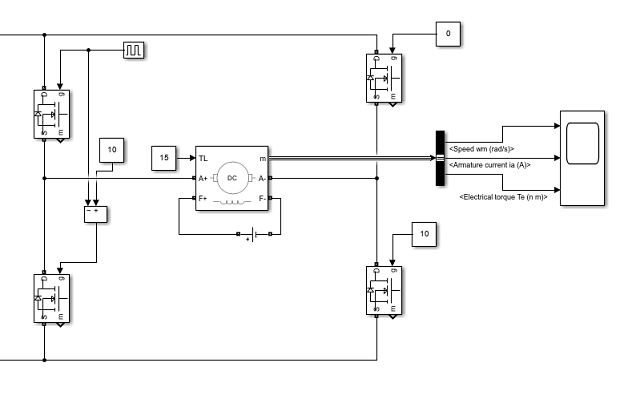
\includegraphics[width=0.8\textwidth]{matlab/MATLAB_model_hbrid.png}
    \caption{MATLAB Simulation Model H-Bridge}
    \label{fig:matlab_model2}
\end{figure}

In this simulation setup, phase-to-phase voltages are given as 150 $V_{rms}$. The output is around 200 $V_{rms}$ with 20 $V_{pp}$ ripple. The H-bridge and DC motor are driven with the output of a three-phase full bridge diode rectifier. Separate simulations are run for motoring, reverse motoring, and regenerative braking modes of operation. In forward motoring, the system works as a synchronous DC-DC buck converter. The output of the forward motoring can be seen in the 50 percent duty cycle in Figure \ref{fig:forward_mot}. The output current is observed to be too much for the system. This is because there is no soft starter simulated. The control part will be implemented later.

\begin{figure}[ht]
    \centering
    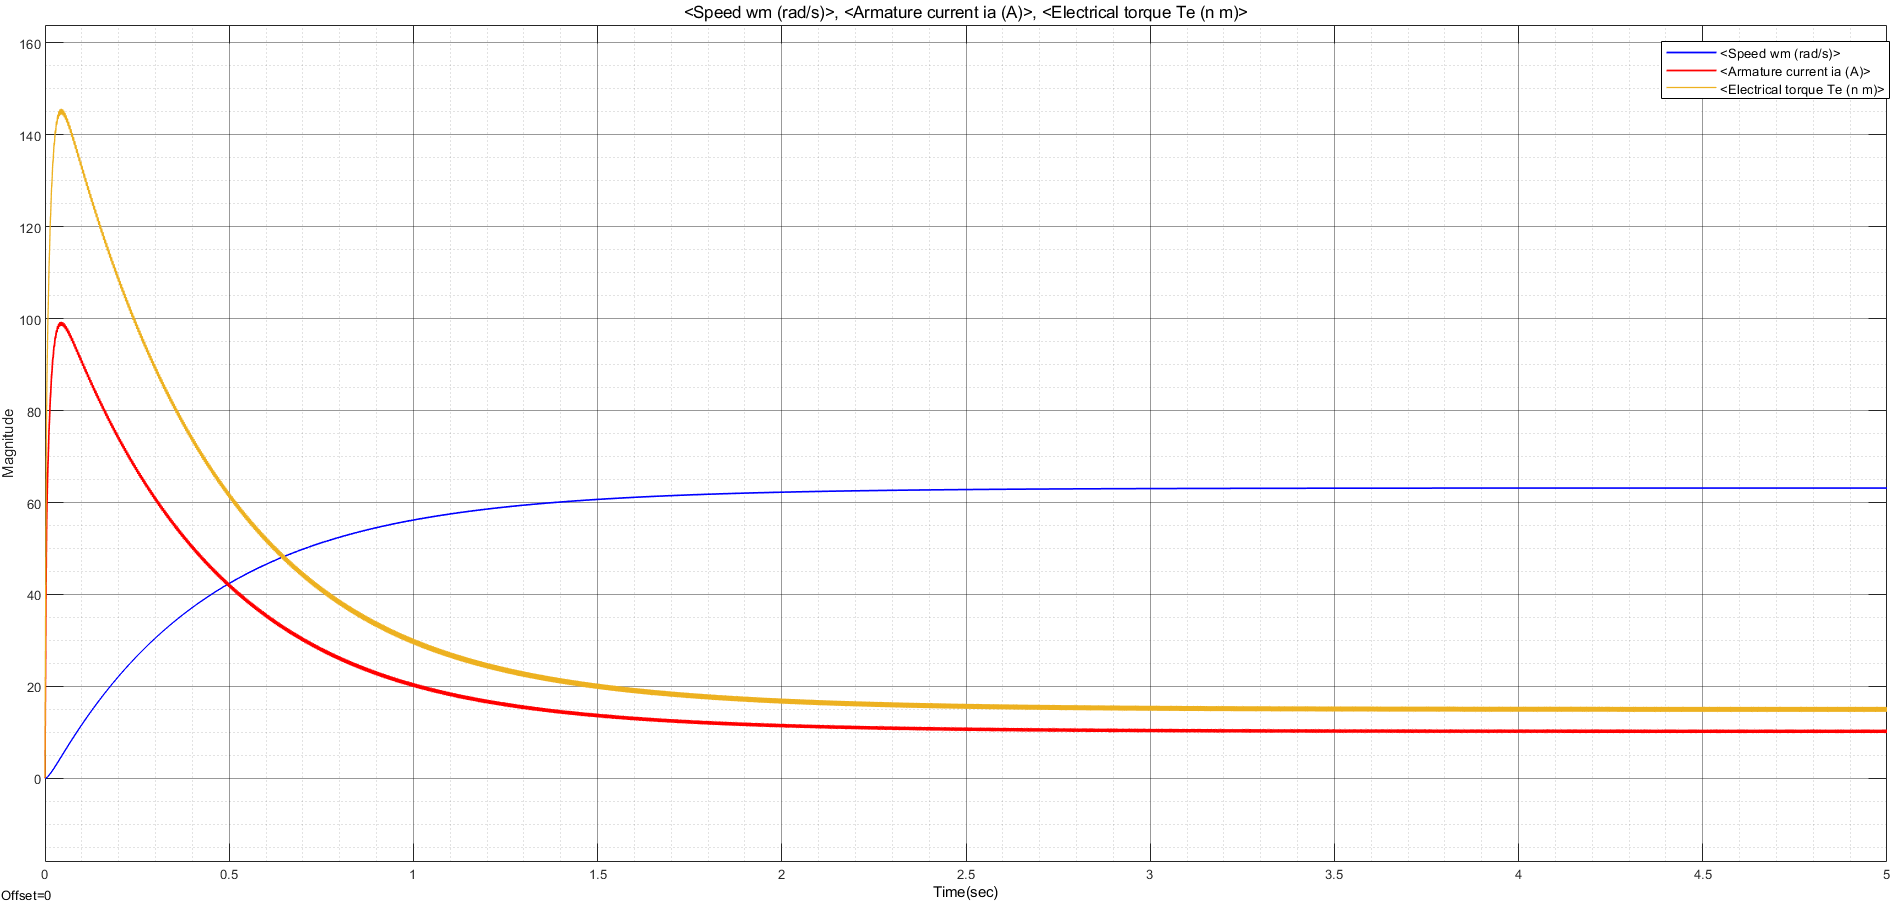
\includegraphics[width=1\textwidth]{matlab/forward motoring D50_900W.png}
    \caption{H-Bridge and DC Motor Simulation at D=0.5 - Forward Motoring}
    \label{fig:forward_mot}
\end{figure}

In Figure \ref{fig:rev_mot}, we see the reverse motoring graph of the motor. It is just the inverted version of forward motoring. The system works with the same logic; however, the controlled MOSFETs are changed due to change of operation. 
\begin{figure}[ht]
    \centering
    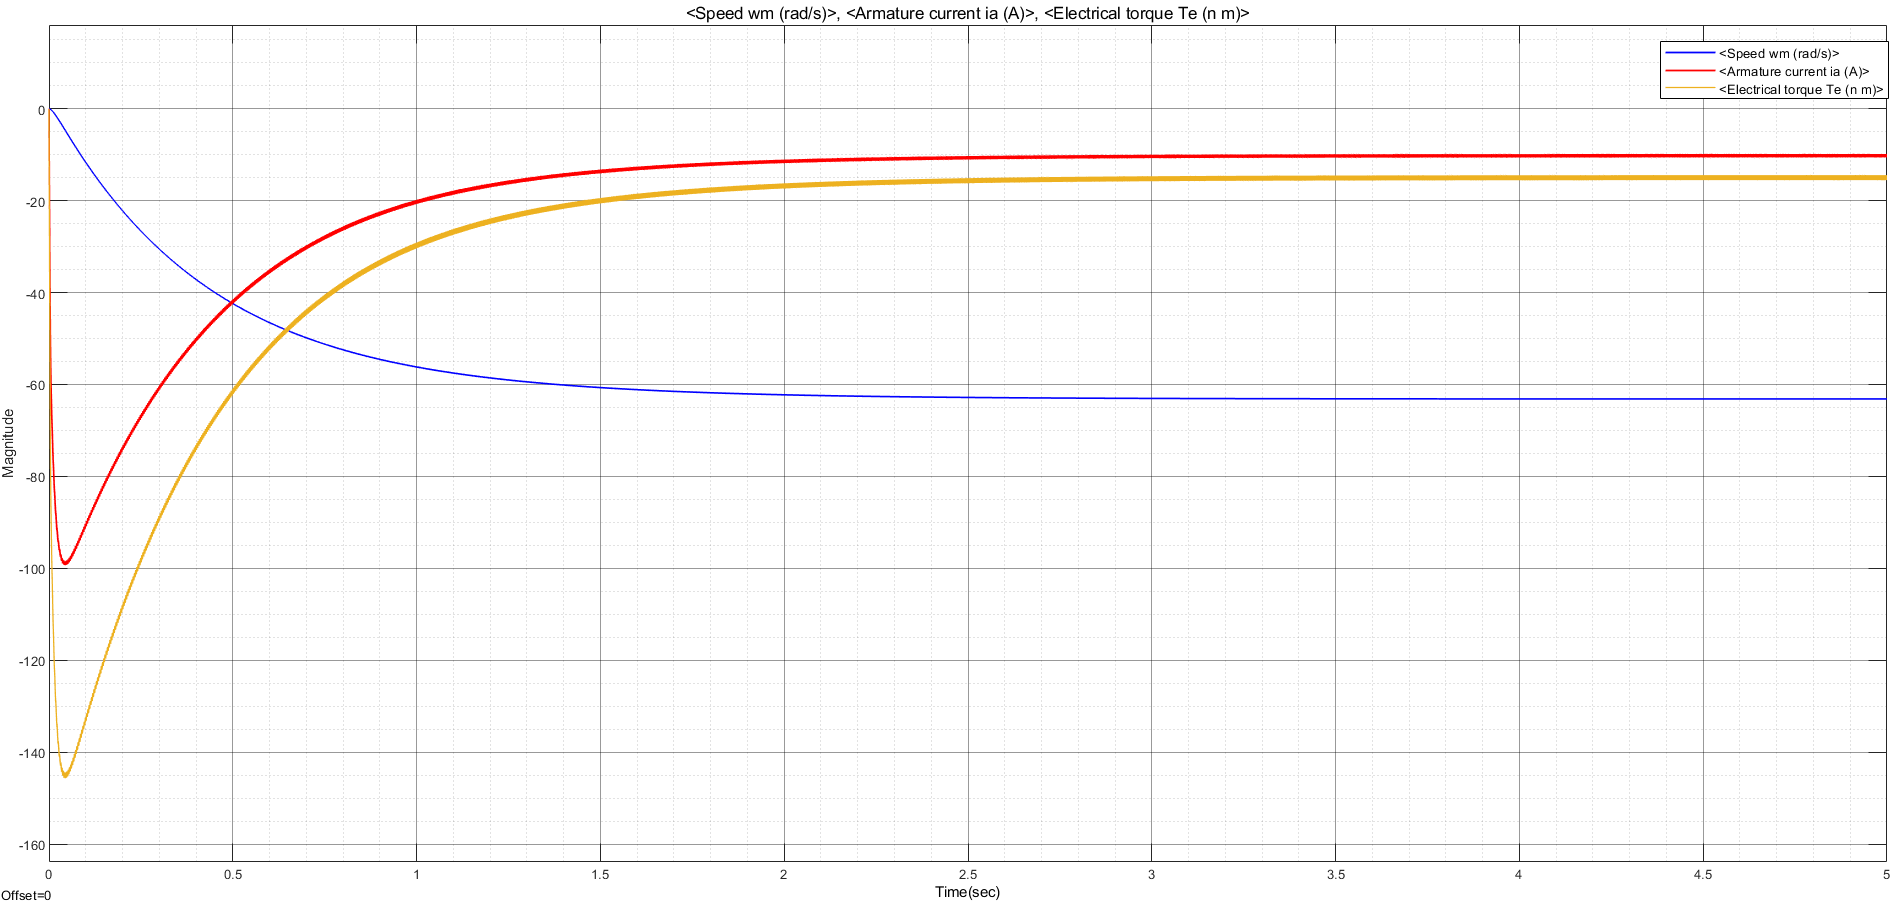
\includegraphics[width=1\textwidth]{matlab/reverse motoring D50_ 900W.png}
    \caption{H-Bridge and DC Motor Simulation at D=0.5 - Reverse Motoring}
    \label{fig:rev_mot}
\end{figure}

The intention of using an H-bridge is to be able to have the four-quadrant drive. More on that topic is explained in Design Decisions[\ref{design}]. The other operation quadrants are braking regions. Braking is simulated in the model by adding a resistor and another MOSFET parallel to the rectifier output as in Figure \ref{fig:braking}.
\newpage
\begin{figure}[ht]
    \centering
    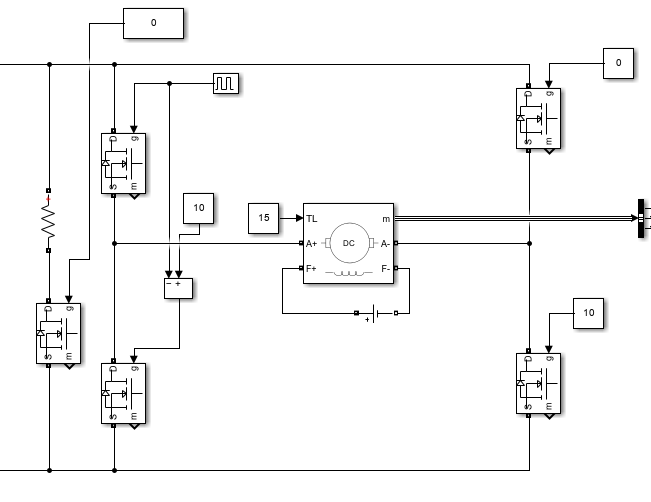
\includegraphics[width=0.8\textwidth]{matlab/braking_added.png}
    \caption{Braking Mode Added Circuitry}
    \label{fig:braking}
\end{figure}

In regenerative braking, the intention is usually to charge a battery system connected to the motor. We will dissipate this external motor energy using a chopper resistor. When it is in braking mode we turn on our MOSFET. More on the operation of the braking mode is explained in Design Decisions[see \ref{design}].

Figure \ref{fig:duty_braking} shows that the current gets below zero, which means our motor injects current into the other direction. This change in the current increases the voltage if not dissipated properly.
\begin{figure}[ht]
    \centering
    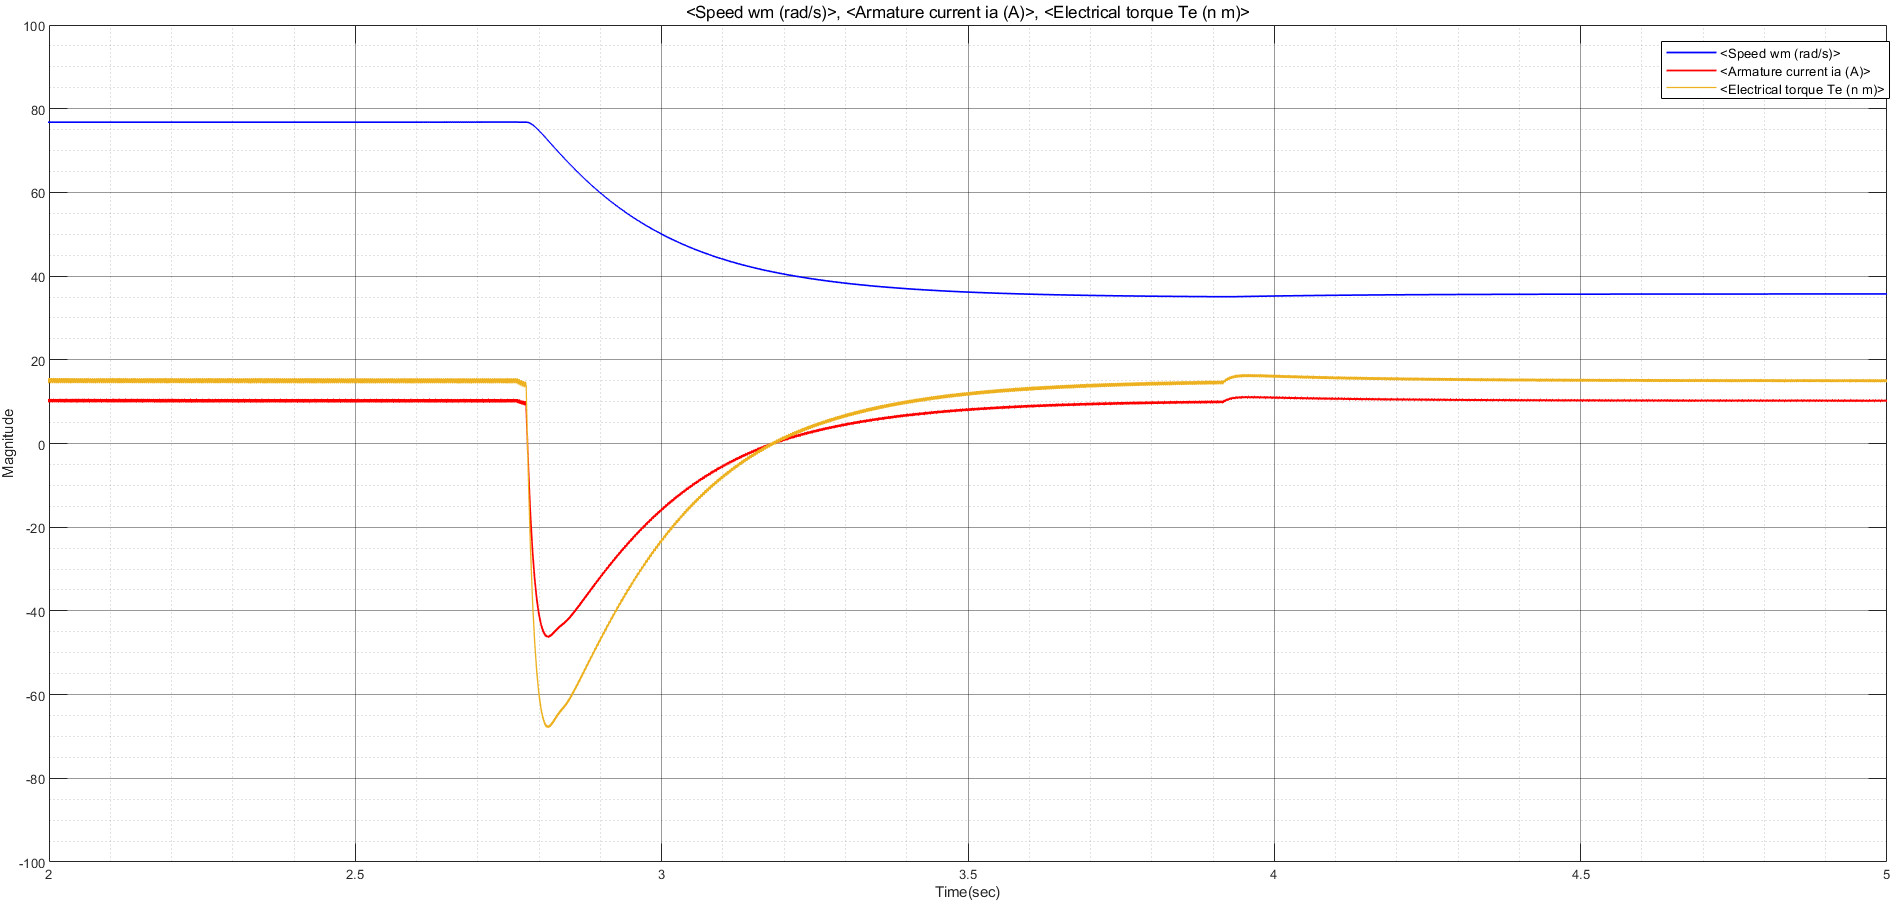
\includegraphics[width=0.9\textwidth]{matlab/braking D60_D30_v2.png}
    \caption{Forward Braking from duty cycle D=0.6 to D=0.3 }
    \label{fig:duty_braking}
\end{figure}